% This document is compiled using pdfLaTeX
% You can switch XeLaTeX/pdfLaTeX/LaTeX/LuaLaTeX in Settings

\documentclass{article}
\usepackage[utf8]{inputenc}
\usepackage{tikz}
\usepackage[hidelinks]{hyperref}
\usepackage{graphicx}
\usepackage{titling}
\usepackage{float}
\usepackage[text={18cm,21cm},centering]{geometry}
\usepackage{enumitem}
\usepackage{amsmath}
\usepackage{graphicx}
\usepackage{xcolor} % Paquete para definir colores
\usepackage{tcolorbox} % Paquete para cuadros de color
\hypersetup{
  colorlinks=true,
  linkcolor=blue,
  urlcolor=blue
}
\usepackage[utf8]{inputenc}
\usepackage{array}
\usepackage{colortbl}
\usepackage{minted}
\usepackage{amssymb}
\usepackage{setspace}
\usepackage{tocbibind}

\title{Title}
\author{Your Name}
\date{\today}

\begin{document}

\maketitle

\tableofcontents

\newpage
\section{Introducción}
Como un problema NP-Completo, por definición, es un problema que es NP y NP hard, la demostración de que un problema es NP-Completo consiste en dos partes:

\begin{itemize}
\item \textbf{Demostrar que es NP:}
Dada una instancia del problema, es posible verificar si es una solución es correcta en tiempo polinomial.
\item \textbf{Demostrar que es NP-Hard:}
Dado un problema NP-Hard conocido B, si B es reducible a C, entonces C es NP-Hard.
\end{itemize}

Ninguno de los problemas planteados a continuación son NP, ya que son problemas de minimizar, y comprobar que un conjunto \(S\) de tamaño \(k\) que cumple con una propiedad \(P\) es mínimo, requiere buscar conjuntos de tamaño menor que  \(k\), y esto es exponencial.

\section{Retroalimentación de arcos}

    \subsection{Definición del problema}
    Dado un grafo $G=(V,E)$, un conjunto de retroalimentación de arcos es un subconjunto de arcos $F \subseteq E$ tal que al eliminar todos los arcos en $F$, el grafo resultante no contiene ciclos (es un grafo acíclico o un bosque, si es no dirigido).

    \textbf{Problema de Optimización}:
    
    El objetivo del problema es encontrar el conjunto de retroalimentación de arcos de tamaño mínimo.

    \textbf{Problema de Decisión}:
    
    El objetivo del problema es ver si existe un conjunto de retroalimentación de arcos de tamaño $k$.
    

\subsection{Demostrar que es NP-Hard}
Reducir \texttt{Cobertura de vértices} a \texttt{Retroalimentación de Arcos}:

La entrada del problema Cobertura de Vértices es un grafo no dirigido $G=(V,E)$. Dado $G=(V,E)$, creamos un grafo dirigido $G'=(V',E')$, tal que:
\begin{itemize}
    \item \(V' = V \cup \{ v' | v \in V\}\)
    \item \(E' = \{ (v,v'),(u,u'), (v',u),(u',v) | <u,v> \in E\}\)
\end{itemize}
Este es la entrada al problema de Retroalimentación de Arcos. A continuación se muestra un ejemplo de ambos grafos.

\begin{figure}[h]
    \centering
    \includegraphics[width=0.3\textwidth]{images/Feedback_arc_set.png}
    \caption{Las aristas amarillas pertenecen a \(G\) y los arcos negros a \(G'\)}
    \label{fig:foto_carpeta}
\end{figure}

\textbf{Correctitud}

Existe una cobertura de vértices en \( G \) de tamaño \(k\) \(\iff\) existe un conjunto de retroalimentación de arcos en \( G' \) de tamaño \(k\).

\begin{itemize}
    \item \(\Leftarrow\) 
    Sea \(S'\) un conjunto de retroalimentación de arcos de \(G'\) de tamaño \(k\), si \(\exists e \in S' \text{ tal que } e \text{ no es una arista }  (v,v') \text{ entonces e es una arista de la forma}  (v',u) \). Si \( e\) es una arista \((v',u)\), como \(e \in S'\), abarca todos los ciclos \( [v',u,...,v']\). Todos los caminos \( u \rightarrow v'\) pasan por \(v\), ya que el único arco incidente en \(v'\) es \(v\). Por tanto si sustituimos \((v',u)\) por \((v,v')\), se abarcan los mismos ciclos de G'. Por tanto, es posible crear un nuevo conjunto \(S'\) de tamaño \(k\) formado solamente por arcos de la forma \((v,v')\). Dado el nuevo conjunto \(S'\), como \(S'\) abarca todos los ciclos, también abarca los ciclos \(c\) de la forma \(c = [v,v',u,u',v]\) en \(G'\). A cada ciclo \(c\) en \(G'\) se le asocia una arista \(<u,v> \in E\) y viceversa. Como por cada ciclo \(c\) \text{se cumple que} \((v,v') \in S' \text{ o } (u,u') \in S'\), entonces es posible crear un conjunto \(S\) formado por los vértices de \(V\) correspondientes a las aristas de \(S'\), el cual abarca todas las aristas de \(G\), por tanto, \(S'\) es una cobertura de vértices de \(G\).
    

    \item \(\Rightarrow\) 
    Sea \(S\) una cobertura de vértices de \(G\), entonces \(\forall <u,v> \in E \text{ se cumple que } u \in S \text{ o } v \in S\). Sea \(S'\) un conjunto de arcos formado por las arcos que \((v',v)\) correspondientes a los vértices \(v\) que pertenecen a S, demostremos que \(G'-S'\) no tiene ciclos. Dado un ciclo \(c\) de \(G'\); si \(v' \in c\ \text{, entonces } (v,v') \in c\), ya que en \(v'\) solo incide \(v\); si \(v \in c\ \text{, entonces } (v,v') \in c\), ya que \(v\) solo incide en \(v'\). Por tanto, en cada ciclo de \(G'\) existe un arco de la forma \((v,v')\), por lo que \(S'\) es una retroalimentación de arcos de \(G'\).
    
    

\end{itemize}

\textbf{Extensión al problema de Optimización}

Existe conjunto de retroalimentación de arcos de tamaño mínimo en \(G\) \(\iff\) existe un conjunto de retroalimentación de arcos en \(G\) de tamaño \(k\), con \(k \geq 0\).
\begin{itemize}
    \item \(\Leftarrow\) 
    Se cumple por Principio del Buen Orden.
    \item \(\Rightarrow\) 
    Si existe un conjunto de retroalimentación de arcos de tamaño mínimo \(l\), al agregar \(k-l\) vértices al conjunto, este va a seguir cumpliendo que es un conjunto de retroalimentación de arcos.
\end{itemize}

\section{Retroalimentación de vértices}

    \subsection{Definición del problema}
    Dado un grafo $G=(V,E)$, un conjunto de retroalimentación de vértices es un subconjunto de vértices $F \subseteq V$ tal que al eliminar todos los vértices en $F$ (y sus aristas incidentes), el grafo resultante no contiene ciclos (es un grafo acíclico o un bosque, si es no dirigido).


    \textbf{Problema de Optimización}:
    
    El objetivo del problema es encontrar el conjunto de retroalimentación de vértices de tamaño mínimo.

    \textbf{Problema de Decisión}:
    
    El objetivo del problema es ver si existe un conjunto de retroalimentación de vértices de tamaño $k$.
    

\subsection{Demostrar que es NP-Hard}
Reducir \texttt{Cobertura de vértices} a \texttt{Retroalimentación de vértices}:

La entrada del problema Cobertura de Vértices es un grafo no dirigido $G=(V,E)$. Dado $G=(V,E)$, creamos un grafo dirigido $G'=(V',E')$, tal que:
\begin{itemize}
    \item \(V' = V\)
    \item \(E' = \{(u,v), (v,u) \quad | \quad  <u,v> \in E\}\)
\end{itemize}
Este es la entrada de la Retroalimentación de vértices. A continuación se muestra un ejemplo de ambos grafos.

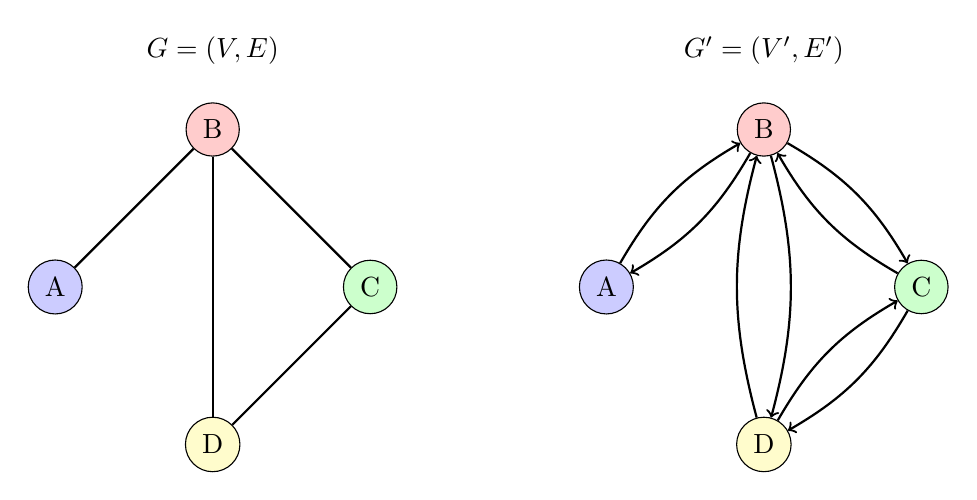
\begin{tikzpicture}
    \node[align=center] at (2, 3) {\textbf{$G=(V,E)$}};
    % Nodos
    \node[circle, draw, fill=blue!20] (A) at (0,0) {A};
    \node[circle, draw, fill=red!20] (B) at (2,2) {B};
    \node[circle, draw, fill=green!20] (C) at (4,0) {C};
    \node[circle, draw, fill=yellow!20] (D) at (2,-2) {D};

    % Aristas
    \draw[thick] (A) -- (B);
    \draw[thick] (B) -- (C);
    \draw[thick] (C) -- (D);
    \draw[thick] (B) -- (D);


     \node[align=center] at (9, 3) {\textbf{$G'=(V',E')$}};
    % Nodos
    \node[circle, draw, fill=blue!20] (A) at (7,0) {A};
    \node[circle, draw, fill=red!20] (B) at (9,2) {B};
    \node[circle, draw, fill=green!20] (C) at (11,0) {C};
    \node[circle, draw, fill=yellow!20] (D) at (9,-2) {D};

    % Aristas
    \draw[thick, ->, bend left = 15] (A) to (B);
    \draw[thick, ->, bend left = 15] (B) to (C);
    \draw[thick, ->, bend left = 15] (C) to (D);
    \draw[thick, ->, bend left = 15] (B) to (D);
    
    \draw[thick, ->, bend left = 15] (B) to (A);
    \draw[thick, ->, bend left = 15] (C) to (B);
    \draw[thick, ->, bend left = 15] (D) to (C);
    \draw[thick, ->, bend left = 15] (D) to (B);

\end{tikzpicture}

\textbf{Correctitud}

Existe una cobertura de vértices en \( G \) de tamaño \(k\) \(\iff\) existe una retroalimentación de vértices en \( G' \) de tamaño \(k\).

\begin{itemize}

\item \(\Leftarrow\)
 Sea \(S'\) una retroalimentación de vértices de tamaño \(k\), entonces \(S'\) contiene al menos un vértice de cada ciclo, entonces \(\forall \text{ ciclo } [u,v,u] \in G' \text{, se cumple que } u \in V' \text{ o } v \in V'\). Como existe un ciclo de este tipo por cada arista de \(G\), entonces \(S'\) cubre todos los vértices de \(G\).

\item \(\Rightarrow\)
Sea \(S\) una cobertura de vértices de tamaño \(k\), entonces \(\forall <u,v> \in E \text{, se cumple que } u \in S \text{ o } v \in S\). Demostremos que \(S\) es una retroalimentación de vértices de \(G'\). Sea \(c\) un ciclo de \(G'\) de tamaño \(q\) \(c\ = [v1,v2,..,vq,v1]\), entonces entre todo par de vértices consecutivos de \(c\) existe un arco \( (vi,vj)\) en \(G'\) y su correspondiente arista \( <vi,vj> \text{ o } <vj,vi> \text{ en } G\). Como \(vi \in S \text{ o }vj \in S\), entonces al menos un vértice de \(c\) pertenece a \(S\), por lo que todos los ciclos de \(G'\) están cubiertos en \(S\).

\end{itemize}

\textbf{Extensión al problema de Optimización}

Existe conjunto de retroalimentación de vértices  de tamaño mínimo en \(G\) \(\iff\) existe un conjunto de retroalimentación de vértices en \(G\) de tamaño \(k\), con \(k \geq 0\).
\begin{itemize}
    \item \(\Leftarrow\) 
    Se cumple por Principio del Buen Orden.
    \item \(\Rightarrow\) 
    Si existe un conjunto de retroalimentación de tamaño mínimo \(l\), al agregar \(k-l\) vértices al conjunto, este va a seguir cumpliendo que para todos los ciclos del grafo existe un vértice en el conjunto, por lo que va a ser un conjunto de retroalimentación de tamaño \(k\).
\end{itemize}

\section{Conjunto Dominante}

    \subsection{Definición del problema}
    En un grafo $G=(V,E)$, un conjunto de vértices $D \subseteq V$ es un conjunto dominante si cada vértice de $V$ que no está en $D$ es adyacente a al menos un vértice en $D$.

    Una partición de los vértices $V$ en $k$ conjuntos $D_1,D_2,…,D_k$ es una partición domática si cada $D_i$ (para $i=1,2,…,k$) es un conjunto dominante. El numero dominante es la cardinalidad del menor conjunto dominante de $G$.

    \textbf{Problema de Optimización}:
    
    Hallar el número dominante de $G$.

    \textbf{Problema de Decisión}:
    
    Ver si existe un conjunto dominanate de tamaño $k$.
    

\subsection{Demostrar que es NP-Hard}
Reducir \texttt{Cobertura de vértices} a \texttt{Conjunto Dominante}:

La entrada del problema Cobertura de Vértices es un grafo no dirigido $G=(V,E)$. Dado $G=(V,E)$, creamos un grafo no dirigido $G'=(V',E')$, tal que:
\begin{itemize}
    \item \(V' = V \cup \{ uv | <u,v> \in E\}\)
    \item \(E' = E \cup \{ <uv,u>, <uv,v> | <u,v> \in E\}\)
\end{itemize}
Este es la entrada al problema de Conjunto Dominante. A continuación se muestra un ejemplo de ambos grafos.

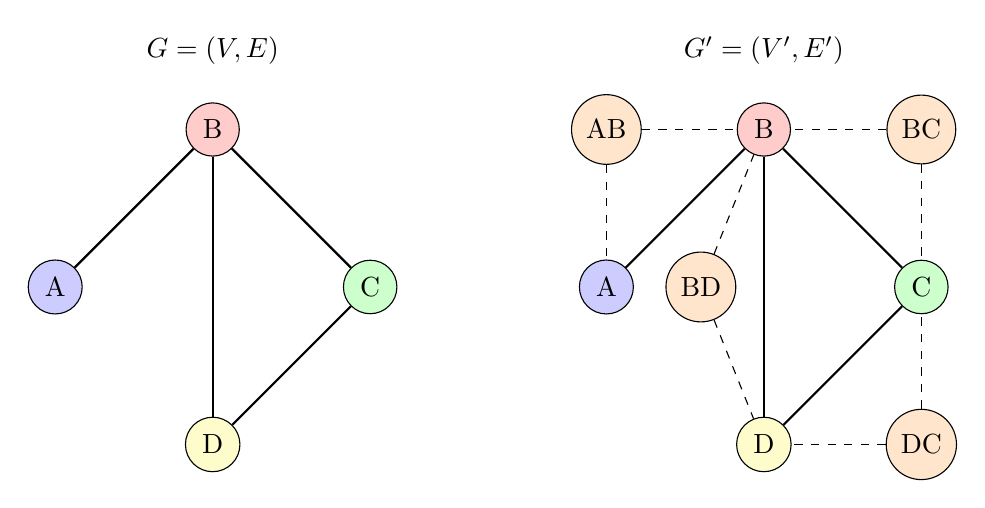
\begin{tikzpicture}
    \node[align=center] at (2, 3) {\textbf{$G=(V,E)$}};
    % Nodos
    \node[circle, draw, fill=blue!20] (A) at (0,0) {A};
    \node[circle, draw, fill=red!20] (B) at (2,2) {B};
    \node[circle, draw, fill=green!20] (C) at (4,0) {C};
    \node[circle, draw, fill=yellow!20] (D) at (2,-2) {D};

    % Aristas
    \draw[thick] (A) -- (B);
    \draw[thick] (B) -- (C);
    \draw[thick] (C) -- (D);
    \draw[thick] (B) -- (D);


     \node[align=center] at (9, 3) {\textbf{$G'=(V',E')$}};
    % Nodos
    \node[circle, draw, fill=blue!20] (A) at (7,0) {A};
    \node[circle, draw, fill=red!20] (B) at (9,2) {B};
    \node[circle, draw, fill=orange!20] (AB) at (7,2) {AB};
    \node[circle, draw, fill=green!20] (C) at (11,0) {C};
    \node[circle, draw, fill=orange!20] (BC) at (11,2) {BC};
    \node[circle, draw, fill=yellow!20] (D) at (9,-2) {D};
    \node[circle, draw, fill=orange!20] (DC) at (11,-2) {DC};
    \node[circle, draw, fill=orange!20] (BD) at (8.2,0) {BD};

    % Aristas
    \draw[thick] (A) -- (B);
    \draw[dashed] (AB) -- (A);
    \draw[dashed] (AB) -- (B);
    \draw[thick] (B) -- (C);
    \draw[dashed] (BC) -- (C);
    \draw[dashed] (BC) -- (B);
    \draw[thick] (C) -- (D);
    \draw[dashed] (DC) -- (D);
    \draw[dashed] (DC) -- (C);
    \draw[thick] (B) -- (D);
    \draw[dashed] (BD) -- (D);
    \draw[dashed] (BD) -- (B);

\end{tikzpicture}

\textbf{Correctitud}

Existe una cobertura de vértices en \( G \) de tamaño \(\k\) \(\iff\) existe un conjunto dominante en \( G' \) de tamaño \(\k\).

\begin{itemize}

\item \(\Leftarrow\)
Sea \(S'\) un conjunto dominante de \(G'\) de tamaño \(k\), si \(\exists x \in S' \text{ tal que } x \notin V \), entonces \x es de la forma \(uv\). Como \(x\) solo es adyacente a \(u\) y a \(v\), significa que \(x\) solo abarcaba a los vértices \(u\), \(v\) y \(x\). Por tanto, al sustituir en \(S'\), \(x\) por \(u\) o \(v\), como los tres vértices forman un triángulo, se siguen abarcando los mismos vértices que se abarcaban inicialmente. Esto significa que es posible obtener un conjunto dominante \(S'\) de tamaño \(k\) formado solamente por vértices v tal que \(v \in V\). 
Dado el nuevo conjunto dominante \(S'\), como los vértices de la forma \(uv \notin S' \) y \(\forall x \text{ tal que } x \notin S' \text{ se cumple que x es adyacente a al menos un vértice de S'}\), entonces por cada vértice de la forma \(uv\), se cumple que \(u \in S' \text{ o } v \in S'\), ya que de no pertenecer ninguno de los dos a \(S'\), no existiría forma de abarcar el vértice \(uv\), ya que este solo es adyacente a esos dos vértices. Por tanto \(S\) es una cobertura de vértices de \(G\) de tamaño \(k\).

\item \(\Rightarrow\) 
Sea \(S\) una cobertura de vértices de tamaño \(k\) de \(G\), entonces \(\forall <u,v> \in E\ \text{ se cumple que } u \in S \text{ o } v \in S}\). Por tanto, todos los vértices que pertenecen a \(V\) y a \(V'\) estarán abarcados en \(G'\). Como los vértices \(x \in V'\) de la forma \(uv\) son adyacentes a \(u\) y a \(v\), y se cumple que \(u \in S \text{ o } v \in S\), estos vértices \(x\) también están siendo abarcados en \(G'\), por lo que \(S\) es un conjunto dominante de \(G'\) de tamaño \(k\).
\end{itemize}

\textbf{Extensión al problema de Optimización}

Existe conjunto dominante de tamaño mínimo en \(G\) \(\iff\) existe un conjunto dominante en \(G\) de tamaño \(k\), con \(k \geq 0\).
\begin{itemize}
    \item \(\Leftarrow\) 
    Se cumple por Principio del Buen Orden.
    \item \(\Rightarrow\) 
    Si existe un conjunto dominante de tamaño mínimo \(l\), al agregar \(k-l\) vértices al conjunto, este va a seguir cumpliendo que es un conjunto dominante.
\end{itemize}



\end{document}
